\documentclass[a4paper, 12pt, oneside]{article}

\usepackage[a4paper, total={140mm, 230mm}]{geometry}
\usepackage[utf8]{inputenc}
\usepackage[italian]{babel}
\usepackage{graphicx}
\usepackage{titling}
\usepackage{fancyhdr}
\usepackage{textgreek}
%\pagestyle{fancy}
%\fancyhead{}
%\fancyhead[R]{\leftmark}
%\fancyfoot{}
\fancyfoot[C]{\thepage}
%\renewcommand{\headrulewidth}{0.4pt}
%\renewcommand{\footrulewidth}{0.4pt}

%per poter usare immagini "concentriche", includere i seguenti packages
\usepackage{caption}
\usepackage{subcaption}
\usepackage{listings}
\usepackage{textcomp}
%per poter includere la bibliografia, includere i seguenti packages
%\usepackage[backend=biber]{biblatex}
\usepackage[
	backend=biber,
	style=numeric
]{biblatex}
\addbibresource{bibliography.bib}

%\usepackage{etoolbox}
%\makeatletter
%\patchcmd{\scr@startchapter}{\if@openright\cleardoublepage\else\clearpage\fi}{}{}{}
%\makeatother

%\usepackage[nottoc, numbib]{tocbibind}
%per poter applicare i cambiamenti alle citazioni, seguire le istruzioni:
%1: compilare il documento da TexStudio
%2: aprire terminale e posizionarsi nella directory che contiene questo file, "main.tex"
%3: lanciare il comando "biber main", senza l'estensione ".tex"
%4: tornare su TexStudio e ricompilare
%Ora la bibliografia dovrebbe essere a posto, con tutte le citazioni.

%per inserire una pagina bianca senza che il numero di pagina aumenti
\usepackage{afterpage}
\newcommand \emptypage{
	\null
	\thispagestyle{empty}
	\addtocounter{page}{-1}
	\newpage
}

%package per referenziare capitoli di questo stesso documento
\usepackage{hyperref}

%imposta la directory in cui trovare le immagini
\graphicspath{{images/}}

%il titolo in questo caso non viene usato (usiamo un frontespizio fornito dall'UPO)
%\title{
%	{Un bellissimo titolo}
	%\author{Lorenzo Rossi}
	%\input{frontespizioLatex/fileConFrontespizio.tex}
	%{\includegraphics{images/upo.jpg}}
	%\date{}
%}


\begin{document}
	%se si lavora con un frontespizio, si può omettere maketitle e mettere in input il file col frontespizio
	%\maketitle
	\begin{titlepage}
	\voffset=8mm
	\begin{center}
%		\includegraphics[width=0.50\textwidth]{../images/logoUPO.png}
		\large{Lorenzo Rossi, matr. 20031485}\\
		\large{Universit\`a degli Studi del Piemonte Orientale}\\
		\large{Dipartimento di Scienze ed Innovazione Tecnologica}\\
		\large{Corso di Laurea Magistrale in Informatica}\\
		\large{Anno Accademico 2020/2021}
		
		\vspace*{1.5cm}
		
		\LARGE{\textbf{Relazione per il progetto del corso di\\Laboratorio di Calcolo}}
			
		%\LARGE{Dipartimento di Scienze e Innovazione Tecnologica}
		
		\vfill
		
		
		
		\vspace*{1.5cm}
		
		\large{Luglio 2021}
	\end{center}
\end{titlepage}
		
	%genera il sommario
	%\tableofcontents
	\newpage
	
	\section{Introduzione}
	\label{intro}
	Si vuole realizzare un programma in linguaggio \textbf{C} con cui valutare il calcolo di un integrale definito di una funzione mediante la generazione di numeri casuali. Il calcolo del valore dell'integrale tramite metodo Monte Carlo avviene attraverso la stima delle aree: vengono generate \textit{n} coppie di valori casuali $(x, y)$ all'interno di un rettangolo che ha come base l'intervallo di integrazione e come altezza la distanza tra $y = 0$ ed il massimo dell'integranda nell'intervallo di integrazione. Conoscendo il valore dell'area del rettangolo ed il numero di punti che cadono tra il grafico dell'integranda e l'asse delle ascisse, è possibile stimare il valore dell'integrale definito con una proporzione.
	
	Una volta scelto un dominio $[a, b]$ ed una funzione limitata in $[a, b]$, è possibile stimarne l'integrale definito in quel dominio sapendo che:
	
	$$\int_{a}^{b}f(x)\,dx\,\approx\,\frac{N_{acc}}{N_{tot}}M(b - a)$$
	dove $N_{acc}$ è il numero di punti generati randomicamente che cadono sotto al grafico di $f(x)$ e che, quindi, vengono ``accettati" (come suggerisce il pedice), mentre $N_{tot}$ è il numero totale di punti generati. $M$ è il massimo valore che $f(x)$ assume in $[a, b]$, ed infine $M(b - a)$ è l'area del rettangolo in cui vengono generati casualmente i punti per valutare l'integrale.
	
	Si è scelto di valutare l'integrale definito della funzione
	$$f(x) = |sin(x)|$$
	
	\newpage
	\section{Struttura del programma}
		\subsection{Funzioni}
			\paragraph{\texttt{double* setRange()}:}
			Questa funzione permette all'utente di impostare il dominio di integrazione. L'utente può scegliere un qualsiasi intervallo all'interno di (0, 10) (estremi esclusi). La funzione restituisce un array bidimensionale che contiene in posizione 0 l'estremo inferiore ed in posizione 1 l'estremo superiore dell'intervallo di integrazione impostato.
			
			\paragraph{\texttt{void setSeed()}:}
			Questa funzione non prevede interazioni con l'utente e viene chiamata prima di generare valori casuali tramite la funzione \texttt{rand()}. Il suo unico scopo è quello di impostare il \textit{seed} per la generazione di numeri casuali, restituito tramite una chiamata interna alla funzione \texttt{time()}, che estrae un seme basandosi sulla data e sull'ora della macchina su cui il programma esegue (più precisamente sulla distanza temporale in secondi dalla mezzanotte del 1\textdegree{} gennaio 1970, detta \textit{epoch} nei sistemi Unix-like). Utilizzando la funzione \texttt{time()} come seed ed essendo il programma di impossibile utilizzo multiplo in meno di un secondo, è ragionevole pensare che due esecuzioni consecutive dello stesso programma si basino su due seed differenti.
			
			\paragraph{\texttt{size\_t setN()}:}
			Questa funzione permette all'utente di scegliere il numero intero di punti da generare all'interno dell'area del rettangolo menzionata nell'Introduzione \ref{intro}, restituendolo per poterlo utilizzare all'interno del programma. Un numero maggiore di punti generati casualmente permette una valutazione più accurata dell'integrale.
			
			\paragraph{\texttt{double getRandomDoubleFromRange(double min, double max)}:}
			Questa\\funzione viene chiamata quando sia necessario generare un valore reale (rappresentato come \texttt{double}) all'interno di un range, definito dall'utente od opportunamente calcolato. Restituisce il \texttt{double} estratto casualmente.
			
			\paragraph{\texttt{double f(double x, double* y\_max)}:}
			Questa funzione può rappresentare una qualsiasi funzione matematica ad una variabile. Dato il parametro \texttt{double x}, restituisce il valore della funzione di cui è fornita l'implementazione all'interno dello scope stesso di \texttt{f()}. Il secondo parametro è un puntatore a \texttt{double} che viene passato per riferimento per poter aggiornare, ad ogni valutazione di $f(x)$, quale sia il massimo di $f(x)$ raggiunto finora. Tale valore sarà utilizzato come altezza del rettangolo in cui è contenuto il grafico di $f(x)$ per poter stimare accuratamente l'integrale definito.
	\newpage
		\subsection{Flowchart}
			\begin{figure}[!htb]
			\begin{minipage}{\textwidth}
				\centering
				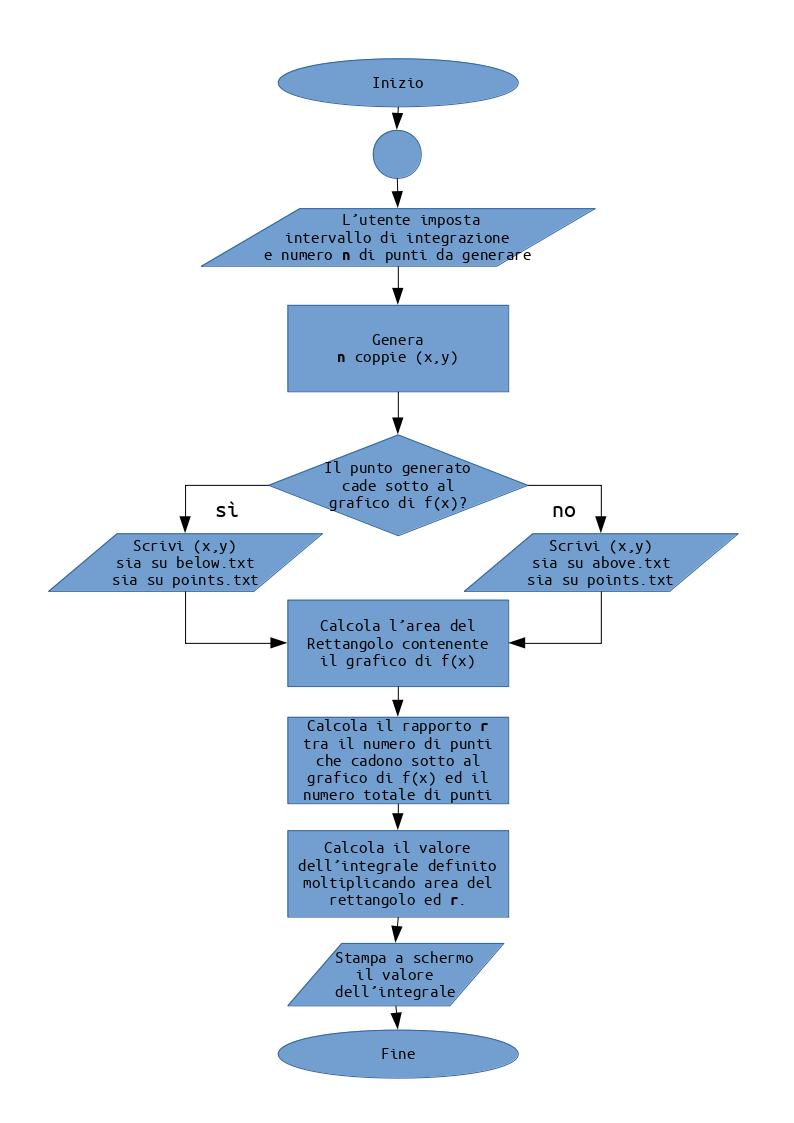
\includegraphics[width=1\linewidth]{flowchart.jpg}
				\caption{Flowchart del programma}
				\label{flowchart}
			\end{minipage}
		\end{figure}
		
		\subsection{Compilazione}
		Dato che il programma si serve della libreria \texttt{math.h} per poter chiamare funzioni matematiche (tra cui \texttt{sin()} e \texttt{fabs()}, che sono state utilizzate nell'implementazione), è necessario compilare il codice istruendo il linked con l'attributo \texttt{-lm}, lanciando dunque un comando seguente da terminale:\\\texttt{gcc "sorgente" -lm -o "eseguibile"}.
	
	\section{Risultati}
	Per verificare il corretto funzionamento del programma, sono stati fatti due esperimenti. In entrambi sono stati mantenuti fissi l'intervallo di integrazione $[0.001, 9.999]$ e la variabilità del seed per la generazione di numeri pseudocasuali.
	
	Per il \textbf{primo esperimento} sono stati utilizzati tre diversi valori di $n$, rispettivamente $10^3$, $10^4$ e $10^5$. I rispettivi grafici disegnati con \textbf{GNUPlot} si possono apprezzare nelle figure \ref{n1000}, \ref{n10000} e \ref{n100000}. I grafici sono stati realizzati singolarmente con il comando \texttt{plot [0:10] 'above.txt' with points, 'below.txt' with points, abs(sin(x))}.
	
	
		\begin{figure}[!htb]
			\centering
			\begin{minipage}{0.45\textwidth}
				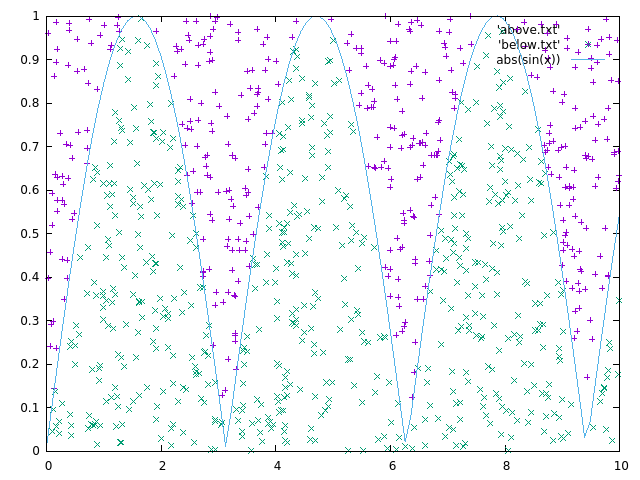
\includegraphics[width=1\linewidth]{n1000.png}
				\caption{$n = 10^3$}
				\label{n1000}
			\end{minipage}
			\hfill
			\begin{minipage}{0.45\textwidth}
				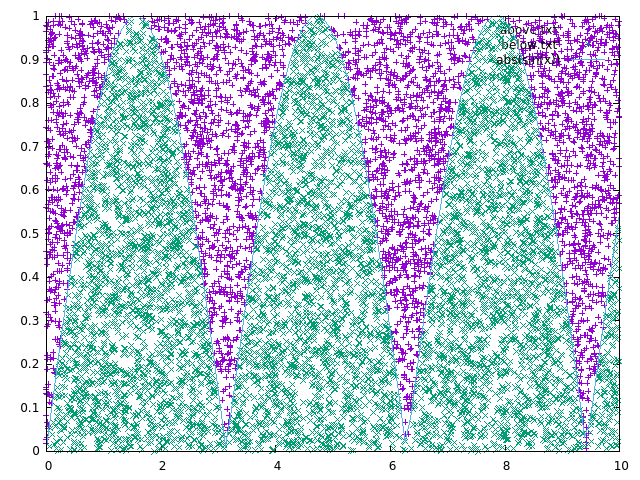
\includegraphics[width=1\linewidth]{n10000.png}
				\caption{$n = 10^4$}
				\label{n10000}
			\end{minipage}
		\end{figure}
	
		\begin{figure}[!htb]
			\centering
			\begin{minipage}{0.45\textwidth}
				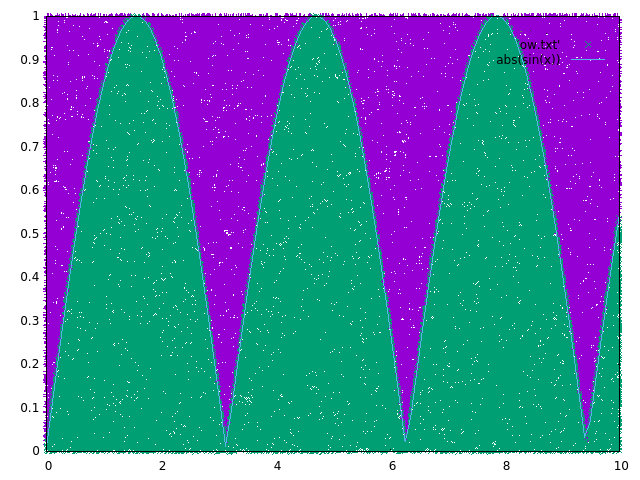
\includegraphics[width=1\linewidth]{n100000.png}
				\caption{$n = 10^5$.}
				\label{n100000}
			\end{minipage}
		\end{figure}
	
	In tutte e tre le immagini, i punti verdi sono evidentemente quelli ``accettati" che cadono sotto al grafico di $f(x)$, raccolti durante l'esecuzione del programma nel file \texttt{below.txt}. I punti viola, invece, sono raccolti nel file \texttt{above.txt} e, sommati ai punti verdi, rappresentano la totalità dei punti generati, anch'essi raccolti nel file \texttt{points\_a\_xmin\_b\_xmax\_n\_N.txt} (dove \texttt{xmin}, \texttt{xmax} e \texttt{N} sono i valori scelti dall'utente rispettivamente per a, b ed n). Si è scelto di scrivere i punti estratti su più files per una visualizzazione più chiara dei punti ``accettati", rispetto ai punti totali, nei grafici GNUPlot.
	
	Da tre iterazioni successive con $n$ ogni volta incrementato di un fattore 10, si ottengono i seguenti valori per l'integrale definito:
	\begin{center}
		\begin{tabular}{|c|c|c|c|}
			\hline
			$n = 10^3$ & $n = 10^4$ & $n = 10^5$ & $``valore\,esatto"*$ \\
			\hline
			5.928793 & 6.257748 & 6.167066 & 6.16038\\
			\hline
		\end{tabular}		
	\end{center}
	
	
	Si nota come, con l'aumentare del numero di punti estratti, diminuisca lo scarto tra il valore esatto dell'integrale e quello stimato mediante metodo Monte Carlo.
	
	Per il \textbf{secondo esperimento}, invece, è stato calcolato 5 volte l'integrale mantenendo fisso $n = 10^5$ e sono stati ottenuti i seguenti risultati:
	
	\begin{center}
		\begin{tabular}{| c | c | c | c | c | c |}
			\hline
			1 & 2 & 3 & 4 & 5 & $``valore\,esatto"*$ \\
			\hline
			6.170866 & 6.151769 & 6.187762 & 6.163167 & 6.129074 & 6.16038\\
			\hline
		\end{tabular}		
	\end{center}
	I valori dell'integrale così calcolati portano ad una deviazione standard $\sigma = 0.01960409915$, grazie a cui è possibile verificare che i valori stimati sono tutti ragionevoli. Trattando $\sigma$ come incertezza sul singolo valore, si ha infatti che il valore esatto cade all'interno di ognuno degli intervalli di incertezza dei valori calcolati.\\
	\textit{(*calcolato con \textbf{WolframAlpha}).}
	
\end{document}